%% UKH thesis and dissertation template (unofficial), following the
%% UKH Presentation Guidelines V6.3 (September 2026).
%%
%% Compile with XeLaTeX and Biber. On Overleaf: Menu > Compiler > XeLaTeX.
%% Class options (put inside [ ]):
%%   numeric   numbered citations [1] instead of APA author-date
%%   eqparens  equation numbers as (3.1) instead of 3.1
%%   nokurdish switch off Sorani Kurdish support
\documentclass{ukhthesis}

%% Your thesis details. main.tex and cover.tex both read this file,
%% so the title page, declaration, certificate and cover always match.

\title{Title of Your Thesis in Title Case}
\subtitle{Subtitle, If Applicable}            % delete the text inside {} if you have none
\author{Your Full Name}
\previousdegree{BSc in Computer Science}      % current degree, shown under your name
\studentid{12345678}

\thesistype{thesis}                           % thesis or dissertation
\degree{Master of Science in Artificial Intelligence}
\degreeshort{MSc}                             % MSc, MA, PhD, BSc ...
\subject{Artificial Intelligence}             % used in the committee certificate

\department{Department of Computer Science and Engineering}
\school{School of Science and Engineering}
\university{University of Kurdistan Hewlêr}

\submissiondate{May 2027}
\place{Erbil, Kurdistan}

\keywords{keyword one, keyword two, keyword three, keyword four}

\addbibresource{references.bib}
\graphicspath{{figures/}}

%% Your own packages and commands go here.
\usepackage{tikz}
\usetikzlibrary{positioning}

\begin{document}

%% ------------------------------------------------ front pages (I, II, III ...)
\frontmatter
\maketitle                      % I   (number not shown)
\makedeclaration                % II
\makecommitteecertification     % III
%% Optional (Guideline 4d). Delete this file's \input line in main.tex if you have none.
\begin{dedication}
To my family, for their patience and support.

\bigskip
Your Name\\
Year
\end{dedication}
        % optional
%% Optional (Guideline 4e).
\begin{acknowledgements}
Thank your supervisor, the people who helped with data or evaluation, your classmates and
your family. Mention any funding or institutional support here.
\end{acknowledgements}
  % optional
%% Guideline 4f: one page, no citations. Key words are set in thesis-info.tex
%% and printed under the abstract automatically.
\begin{abstract}
State the problem and why it matters. Describe how you investigated it: the data, methods
and evaluation. Give the main results with numbers, and the contribution your work makes to
knowledge in the field. End with the main conclusion.

Keep it to a single page of A4. Do not include citations or references.
\end{abstract}

\tableofcontents
\listoftables                   % delete if you have no tables
\listoffigures                  % delete if you have no figures
%% Guideline 4h: alphabetical order. One line per abbreviation: short form & meaning \\
\begin{abbreviations}
AI   & Artificial Intelligence \\
LLM  & Large Language Model \\
NLP  & Natural Language Processing \\
RAG  & Retrieval-Augmented Generation \\
UKH  & University of Kurdistan Hewlêr \\
\end{abbreviations}
     % delete if not needed
%% Guideline 4h: alphabetical order. Use math mode for symbols.
\begin{symbols}
$k$        & Number of retrieved documents \\
$q$        & A query \\
$\theta$   & Model parameters \\
\end{symbols}
           % delete if not needed

%% ------------------------------------------------ chapters (1, 2, 3 ...)
\mainmatter
%% Guideline 5a: Chapter 1 must be the Introduction and be labelled so.
\chapter{Introduction}
\label{ch:introduction}

This chapter introduces the topic. It gives the background to the problem so that readers
understand why the work matters, relates the thesis to other work in the field, and points
to the main findings and contributions.

Write paragraphs as normal text with a blank line between them. The template adds the space
between paragraphs and the one and a half line spacing for you, so never add manual spacing.

\section{Problem Statement}
State clearly the problem your work answers. Keep it focused and concise.

\section{Objectives}
List specific, measurable and achievable objectives, for example:
\begin{enumerate}
  \item Build a test set for the task.
  \item Compare two or more methods on that test set.
  \item Analyse where each method succeeds and fails.
\end{enumerate}

\section{Thesis Organisation}
Give a short description of each chapter. Chapter~\ref{ch:literature} reviews related work,
Chapter~\ref{ch:methodology} describes the method, Chapter~\ref{ch:experiments} the
experiments, Chapter~\ref{ch:results} the results and Chapter~\ref{ch:conclusions} the
conclusions.

\section{Summary}
Each chapter may end with a short summary (optional).

\chapter{Literature Review}
\label{ch:literature}

The literature review tells the story of the work your thesis builds on. Group studies by
theme, compare them, and show the gap that your work fills.

\section{Citing Sources with Page Numbers}
UKH requires a page number in every in-text citation, whatever the referencing style
(Guideline 1c). Put the page in square brackets before the key:

\begin{verbatim}
\parencite[p.~9461]{lewis2020rag}
\textcite[p.~425]{jarvelin2002cumulated}
\parencite[pp.~758--759]{cormack2009reciprocal}
\end{verbatim}

These give \parencite[p.~9461]{lewis2020rag}, then \textcite[p.~425]{jarvelin2002cumulated},
and \parencite[pp.~758--759]{cormack2009reciprocal}.

Direct quotations longer than about forty words go in a \texttt{quote} environment, which
is single spaced as the guidelines require:

\begin{quote}
An indented quotation is set with single line spacing, as Guideline 3d asks. Give the
source and page number at the end \parencite[p.~2]{mahmudi2023meter}.
\end{quote}

\section{Writing Kurdish Text}
Sorani Kurdish in Arabic script works out of the box. Inside an English sentence use
\verb|\textkurdish{...}|, for example \textkurdish{زانکۆی کوردستان هەولێر}
(University of Kurdistan Hewlêr). For a whole right-to-left paragraph, such as a quoted
line of poetry, use the \texttt{kurdish} environment:

\begin{kurdish}
ئەمە نموونەیەکە بۆ نووسینی دەقی کوردی لە ناو نامەی ماستەردا.
پیتە تایبەتەکانی کوردی: ڕ ڵ ێ ۆ ە ڤ.
\end{kurdish}

Kurdish studies relevant to this kind of work include information retrieval
\parencite[p.~3]{esmaili2014kurdish} and poetry analysis \parencite[p.~1]{mahmudi2023meter}.

\section{Summary}
Summarise the gap in the literature that your thesis addresses.

%% The guideline calls this chapter "Theoretical Approach"; rename it to suit your work.
\chapter{Methodology}
\label{ch:methodology}

Describe the theory, design and methods of your work in enough detail for someone else to
repeat it.

\section{Equations}
Write equations with LaTeX, never paste them as images (Guideline 6b). Each equation sits
on its own line and is numbered within the chapter:
\begin{equation}
  \mathrm{nDCG}@k = \frac{1}{\mathrm{IDCG}@k}\sum_{i=1}^{k}\frac{2^{rel_i}-1}{\log_2(i+1)}
  \label{eq:ndcg}
\end{equation}
Refer to it in the text as equation~\ref{eq:ndcg}.

\section{Figures}
Figures are numbered within the chapter and their captions are centred underneath, in
10~pt type (Guideline 6a). Figure~\ref{fig:pipeline} is drawn with TikZ; for an image file,
put it in the \texttt{figures} folder and use \verb|\includegraphics|.

\begin{figure}[htbp]
  \centering
  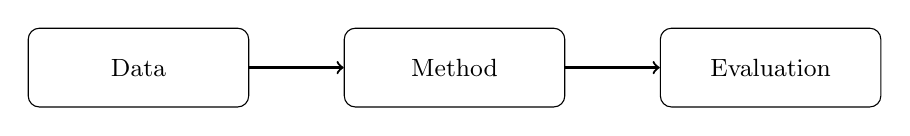
\begin{tikzpicture}[node distance=1.2cm,
      box/.style={draw,rounded corners,minimum width=2.8cm,minimum height=1cm,
                  align=center,font=\small}]
    \node[box] (data) {Data};
    \node[box,right=of data] (method) {Method};
    \node[box,right=of method] (eval) {Evaluation};
    \draw[->,thick] (data) -- (method);
    \draw[->,thick] (method) -- (eval);
  \end{tikzpicture}
  \caption{The three stages of the study}
  \label{fig:pipeline}
\end{figure}

\subsection{Sub-sections}
Sub-sections are numbered 3.2.1, 3.2.2 and so on. The guidelines allow no deeper
numbering; use bullet points instead.

\section{Summary}
Summarise the method.

\chapter{Experimental Work}
\label{ch:experiments}

Describe the data, the experimental set-up and the evaluation measures.

\section{Tables}
Table captions are centred above the table in 10~pt type, and the table text is single
spaced (Guidelines 3d and 6a). Keep tables within the text width; put a very wide table on
its own landscape page.

\begin{table}[htbp]
  \centering
  \caption{Example of a results table}
  \label{tab:example}
  \begin{tabular}{@{}lccc@{}}
    \toprule
    Method        & Recall@5 & MRR@10 & nDCG@10 \\
    \midrule
    Keyword (BM25) & 0.82    & 0.71   & 0.74 \\
    Embedding      & 0.64    & 0.52   & 0.57 \\
    Hybrid         & 0.86    & 0.75   & 0.78 \\
    \bottomrule
  \end{tabular}
\end{table}

Refer to tables in the text as table~\ref{tab:example}.

\section{Summary}
Summarise the experimental set-up.

\chapter{Results and Discussion}
\label{ch:results}

Present the results, then explain what they mean, why they came out this way, and how they
compare with earlier work.

\section{Main Results}
Report numbers with their tests of significance where appropriate.

\section{Discussion}
Discuss strengths, weaknesses and threats to validity.

\section{Summary}
Summarise the findings.

\chapter{Conclusions and Recommendations}
\label{ch:conclusions}

\section{Conclusions}
Answer the objectives from Chapter~\ref{ch:introduction} one by one.

\section{Recommendations and Future Work}
Suggest what should be done next.


%% ------------------------------------------------ end pages (R1, G1, A1 ...)
\references                     % R1, R2 ...
%% Guideline 8b: alphabetical list of technical terms as used in your thesis.
\begin{glossaryterms}
  \item[Corpus] A large, structured collection of texts used for study or training.
  \item[Embedding] A list of numbers that represents the meaning of a text.
  \item[Retrieval] Finding the documents most relevant to a query.
\end{glossaryterms}
            % G1 ... delete if not needed
\appendix                       % A1, A2 ...
%% Guideline 8c: the Ethical Consent Approval form must be one of the appendices.
\chapter{Ethical Consent Approval Form}
\label{app:ethics}

Insert the signed Ethical Consent Approval form here, for example as a scanned PDF:

% \includegraphics[width=\textwidth]{figures/ethics-form.pdf}
   % the Ethical Consent Approval form is required
\chapter{Additional Material}
\label{app:extra}

Appendices hold long supporting material that would interrupt the main text, such as
questionnaires, full result tables or code listings.

\section{Long Appendix Sections}
Sections inside an appendix are numbered Appendix 2.1, 2.2 and so on, and appear in the
table of contents.


\end{document}
